% !TeX spellcheck = pt_BR
\documentclass[12pt,portuguese]{article}

%----------------------------------------------------------------------
% PACOTES ESSENCIAIS E TRADUÇÃO
%----------------------------------------------------------------------
\usepackage[brazilian]{babel}     % Suporte à língua portuguesa
\usepackage[utf8]{inputenc}       % Codificação de entrada
\usepackage[T1]{fontenc}          % Codificação da fonte
\usepackage{lmodern}              % Fonte escalável

%----------------------------------------------------------------------
% PACOTES MATEMÁTICOS
%----------------------------------------------------------------------
\usepackage{amsmath, amsthm, amssymb, amstext, mathtools}
\usepackage{mathrsfs}             % Para fontes como \mathscr
\usepackage{dsfont}               % Para o indicador de conjunto \mathds{1}
\usepackage[all]{xy}              % Para diagramas comutativos
\usepackage{imakeidx}             % Criação de Lista de Símbolos / Índice

% Desigualdades sempre com símbolos inclinados
\let\leq\leqslant
\let\le\leqslant
\let\ge\geqslant
\let\geq\geqslant

%----------------------------------------------------------------------
% FORMATAÇÃO, LAYOUT E CORES
%----------------------------------------------------------------------
\usepackage{geometry}
\usepackage{varwidth}
\usepackage{graphicx}
\usepackage[pdftex]{xcolor}
\usepackage{titlesec}
\usepackage{appendix}
\usepackage{enumitem}
\usepackage{float}
\usepackage{booktabs}
\usepackage{array}
\usepackage{colortbl}
\usepackage{fontawesome5}
\usepackage{lucide-icons}
\usepackage{caption}
\usepackage{stackengine}
\captionsetup{width=0.8\textwidth}

% Definição de Cores
\definecolor{teal}{RGB}{15,118,110}
\definecolor{text}{RGB}{28,25,23}
\definecolor{muted}{RGB}{87,83,78}
\definecolor{card}{RGB}{255,255,255}
\definecolor{border}{RGB}{231,229,228}

% Definição de margens e espaçamento
\setlength{\topmargin}{-0.7in}
\setlength{\oddsidemargin}{0in}
\setlength{\textheight}{9.55in}
\setlength{\textwidth}{6.5in}
\setlength{\baselineskip}{12mm}

% Formatação dos títulos de seção
\titleformat{\section}{\Large\bfseries}{\thesection.}{0.5em}{}
\titleformat{\subsection}{\large\bfseries}{\thesubsection.}{0.5em}{}
\titleformat{\subsubsection}{\normalfont\itshape}{\thesubsubsection.}{0.6em}{}

%----------------------------------------------------------------------
% TIKZ E GRÁFICOS
%----------------------------------------------------------------------
\usepackage{tikz}
\usepackage{pgfplots}
\pgfplotsset{compat=1.17}
\usetikzlibrary{positioning,calc,fit,nfold,decorations.pathreplacing,calligraphy,tikzmark,patterns,arrows.meta,bending,hobby}

%----------------------------------------------------------------------
% REFERÊNCIAS, LINKS E METADADOS DO PDF
%----------------------------------------------------------------------
\usepackage[pdftex, colorlinks, linkcolor={red!50!black}, 
citecolor={red}, urlcolor={blue!80!black}]{hyperref}

\hypersetup{
pdftitle={Densidades Condicionais},
pdfauthor={L. Cioletti},
pdfsubject={Densidade condicional, condicionamento em eventos de probabilidade nula, função de distribuição condicional, fórmula de Bayes para densidades, normal bivariada},
pdfkeywords={densidade condicional, probabilidade condicional, função de distribuição condicional, fórmula de Bayes, normal bivariada, MAT-UnB}
}

% --- PACOTE E COMANDO PARA A LICENÇA CREATIVE COMMONS ---
\usepackage[type={CC},modifier={by-nc-sa},version={4.0}]{doclicense}
\newcommand\blfootnote[1]{%
\begingroup
\renewcommand\thefootnote{}\footnote{#1}%
\addtocounter{footnote}{-1}%
\endgroup
}

%----------------------------------------------------------------------
% ALIASCNT E AMBIENTES DE TEOREMA (Cleveref)
%----------------------------------------------------------------------
\usepackage{aliascnt}
\theoremstyle{definition}
\newtheorem{theorem}{Teorema}

\newaliascnt{definition}{theorem}
\newtheorem{definition}[definition]{Definição}
\aliascntresetthe{definition}

\newaliascnt{example}{theorem}
\newtheorem{example}[example]{Exemplo}
\aliascntresetthe{example}

\newaliascnt{proposition}{theorem}
\newtheorem{proposition}[proposition]{Proposição}
\aliascntresetthe{proposition}

\newaliascnt{corollary}{theorem}
\newtheorem{corollary}[corollary]{Corolário}
\aliascntresetthe{corollary}

\newaliascnt{lemma}{theorem}
\newtheorem{lemma}[lemma]{Lema}
\aliascntresetthe{lemma}

\newaliascnt{remark}{theorem}
\newtheorem{remark}[remark]{Observação}
\aliascntresetthe{remark}

\newtheoremstyle{plainexercise}
  {3pt}{3pt}{\normalfont}{}{\bfseries}{.}{.5em}
  {\thmnumber{#2}\thmnote{ #3}}
\theoremstyle{plainexercise}
\newtheorem{exercise}{Exercício}

% Versão marcada dos exercícios: a estrela fica pendurada na margem esquerda,
% como nas notas anteriores.
\newtheoremstyle{starredexercise}
  {3pt}{3pt}{\normalfont}{}{\bfseries}{.}{.5em}
  {\llap{\textasteriskcentered\,}\thmnumber{#2}\thmnote{ #3}}
\theoremstyle{starredexercise}
\newtheorem{starredexercise}[exercise]{Exercício}
\theoremstyle{definition}

% Ambientes não numerados usados no texto
\newtheorem*{property}{Propriedade}
\newtheorem*{solution}{Solução}

% Se um enumerate for o primeiro conteúdo de um teorema/exercício (cabeçalho
% ainda pendente, \@inlabel true), o \leavevmode dispara o \everypar do amsthm
% que coloca o cabeçalho na própria linha, antes da lista iniciar.
\makeatletter
\setlist[enumerate]{before={\if@inlabel\leavevmode\fi}}
\makeatother

% Nomes em português para os ambientes
\AtBeginDocument{\renewcommand{\proofname}{\normalfont\textbf{Prova}}}
\renewcommand{\qedsymbol}{$\blacksquare$}

% Cleveref (deve vir depois de hyperref e amsthm)
\usepackage[brazilian,nameinlink]{cleveref}

\crefname{theorem}{teorema}{teoremas}
\Crefname{theorem}{Teorema}{Teoremas}
\crefname{definition}{definição}{definições}
\Crefname{definition}{Definição}{Definições}
\crefname{lemma}{lema}{lemas}
\Crefname{lemma}{Lema}{Lemas}
\crefname{proposition}{proposição}{proposições}
\Crefname{proposition}{Proposição}{Proposições}
\crefname{corollary}{corolário}{corolários}
\Crefname{corollary}{Corolário}{Corolários}
\crefname{example}{exemplo}{exemplos}
\Crefname{example}{Exemplo}{Exemplos}
\crefname{exercise}{exercício}{exercícios}
\Crefname{exercise}{Exercício}{Exercícios}
\crefname{remark}{observação}{observações}
\Crefname{remark}{Observação}{Observações}
\crefname{section}{seção}{seções}
\Crefname{section}{Seção}{Seções}

%----------------------------------------------------------------------
% MACROS ADICIONAIS
%----------------------------------------------------------------------
\let\oldemptyset\emptyset
\let\emptyset\varnothing
\graphicspath{{./}{../arquivos-aux/}}

% Seno na convenção em português
\renewcommand{\sin}{\operatorname{sen}}

\begin{document}
% --- CABEÇALHO COM O LOGO DA UnB ---
\vspace*{-0.8cm}
\begin{figure}[H]

\includegraphics{logo-mat-unb.pdf}
\end{figure}


% --- TÍTULO, AUTOR E DATA ---
\vspace*{0.3cm}
\begin{center}
{\LARGE\bf Densidades Condicionais}
\vspace{1cm}

{\large \bf L. Cioletti}
\vspace{0.3cm}

{\footnotesize Outubro de 2026}
\end{center}

% --- RESUMO (ABSTRACT) ---
\begin{abstract}
Nestas notas estudamos a densidade condicional de um par de variáveis
aleatórias conjuntamente contínuas. O ponto de partida é a dificuldade de
atribuir sentido à expressão $\mathbb{P}(Y \leqslant y \mid X = x)$ pela
fórmula usual de probabilidade condicional, já que o evento $\{X = x\}$ tem
probabilidade zero quando $X$ possui densidade. Resolvemos o problema
condicionando na faixa $x \leqslant X \leqslant x+\delta x$ e passando ao
limite quando $\delta x \downarrow 0$, o que produz a função de distribuição
condicional $G$ e a densidade condicional
$f_{Y\mid X}(y\mid x) = f_{X,Y}(x,y)/f_X(x)$. Mostramos que a função assim
definida é de fato uma densidade de probabilidade e discutimos a
independência, a fórmula de Bayes para densidades e o fato de que a densidade
condicional fica determinada apenas em quase todo ponto. Desenvolvemos três
exemplos: uma densidade conjunta sobre o domínio triangular $0 < x < y$, a
normal bivariada, cuja densidade condicional é novamente normal, e a densidade
uniforme sobre um triângulo. Propomos também exercícios, alguns resolvidos,
que fixam a definição e o cálculo das densidades condicionais. A exposição
segue de perto a Seção 6.6 e parte da Seção 6.8 do Capítulo 6 da referência
\cite{GrimmettWelsh2014}.
\end{abstract}

% --- LICENÇA NO RODAPÉ ---
\blfootnote{%
\doclicenseImage[imagewidth=2.6em]\ 
\begingroup
\hypersetup{urlcolor=darkgray}
\href{\doclicenseURL}{%
\doclicenseName - Attribution-NonCommercial-ShareAlike 4.0 International%
}%
\endgroup
}

%----------------------------------------------------------------------
% CONTEÚDO
%----------------------------------------------------------------------

\section{Introdução}\label{sec:introducao}

Nas notas anteriores sobre vetores contínuos aprendemos a descrever o comportamento
conjunto de um par de variáveis aleatórias $(X,Y)$ absolutamente contínuo por meio de sua
densidade conjunta $f_{X,Y}$ e vimos como recuperar as distribuições marginais integrando
a densidade conjunta na coordenada restante. Aqui damos o passo seguinte: descrever a
distribuição de $Y$ quando recebemos alguma informação sobre o valor assumido por $X$.
Esse é o problema central destas notas. A partir da densidade conjunta, queremos atribuir
um sentido preciso à expressão ``distribuição condicional de $Y$ dado que $X = x$'' e
obter uma densidade que a represente. Como veremos, a densidade condicional em $x$
depende apenas dos valores de $f_{X,Y}(x,\cdot)$ e de $f_X(x)$, o que torna o cálculo
simples depois que a definição correta é estabelecida.

Vamos começar recordando o que a densidade marginal representa. Suponha que estamos interessados 
apenas em $Y$ e que nenhuma informação sobre o valor assumido por $X$ seja dada. Neste caso,
podemos recuperar a distribuição de $Y$ simplesmente integrando a densidade conjunta sobre todos 
os valores possíveis de $X$, isto é,
\[
  f_Y(y) = \int_{-\infty}^{\infty} f_{X,Y}(x,y)\,dx,
\]
nos pontos em que essa integral é finita. No caso discreto, o procedimento análogo seria somar
sobre todos os valores possíveis que a variável aleatória $X$ assume, ou seja,
$\sum_x \mathbb{P}(X = x,\, Y = y)$.
Em outras palavras, se não há disponível nenhuma informação sobre $X$, 
a descrição da distribuição de $Y$ é dada simplesmente pela marginal
$f_Y$.

\bigskip 
Consideremos agora a situação oposta, na qual temos informação completa sobre o valor
assumido por $X$. Suponha que nos seja informado que $X$ assume o valor $x$. Essa
informação altera, em princípio, a distribuição de $Y$, e queremos descrever a
``distribuição condicional de $Y$ dado que $X = x$''. A primeira tentativa seria usar a
fórmula usual de probabilidade condicional,
\[
  \mathbb{P}(A \mid B) = \frac{\mathbb{P}(A \cap B)}{\mathbb{P}(B)},
\]
aplicada a $A = \{Y \leqslant y\}$ e $B = \{X = x\}$. Essa tentativa fracassa, e vale a
pena entender exatamente por quê. Como $X$ é uma variável aleatória absolutamente
contínua, o evento $\{X = x\}$ tem probabilidade zero, ou seja, $\mathbb{P}(X = x) = 0$.
Esse fato já foi discutido nas notas sobre funções de distribuição: a probabilidade de
qualquer ponto isolado é nula para variáveis com densidade. Assim, a fórmula acima
envolveria uma divisão por zero.


\bigskip 

A ideia que resolve o problema é substituir o evento exato $\{X = x\}$, de probabilidade
nula, por um evento de probabilidade positiva que o aproxima, a saber, o evento
$\{x \leqslant X \leqslant x+\delta x\}$, com $\delta x > 0$ e pequeno. 
Por questão de clareza, vamos assumir que a função de densidade $f_X$
seja contínua no ponto $x$ considerado e que $f_X(x)>0$.
Neste caso, segue das propriedades elementares da integral de Riemann que a probabilidade
$\mathbb{P}(x \leqslant X \leqslant x+\delta x)$ é aproximadamente $f_X(x)\,\delta x$ e consequentemente
positiva. Desta forma podemos apelar para a definição usual de probabilidade condicional 
para obter a fórmula para a densidade condicional.
Voltaremos a discutir os detalhes destas observações ao longo da prova da \Cref{prop:limite-faixa}. 

\bigskip 

Sob as condições impostas acima, a probabilidade condicional
$\mathbb{P}(Y \leqslant y \mid x \leqslant X \leqslant x+\delta x)$ está bem definida
para $\delta x > 0$ suficientemente pequeno. Nosso objetivo
será estudar o seu comportamento quando $\delta x \downarrow 0$. É esse limite, e não a razão de
probabilidades original, que dará sentido à distribuição condicional de $Y$ dado
$X = x$. A \Cref{fig:faixa-condicionamento} mostra a faixa de condicionamento e a região
do plano envolvida nesse cálculo. Nas próximas seções, executamos essa ideia passo a
passo: primeiro derivamos o limite com cuidado, depois formulamos a definição de
densidade condicional, em seguida estabelecemos suas primeiras propriedades e, por fim,
apresentamos exemplos e exercícios que fixam a definição.

\begin{figure}[H]
\centering
\begin{tikzpicture}[scale=1.0, transform shape=false, >=Stealth]
  % Faixa x <= X <= x+dx: tom claro para todos os valores de Y, tom escuro para Y <= y.
  %\fill[teal!12] (1.8,0) rectangle (3.0,4.3);
  \fill[teal!38] (1.8,-2) rectangle (3.0,2.0);
  \draw[teal, line width=0.8pt] (1.8,-2) -- (1.8,4.3);
  \draw[teal, line width=0.8pt] (3.0,-2) -- (3.0,4.3);

  % Eixos.
  \draw[->, line width=0.8pt] (-1.3,0) -- (8.0,0) node[below] {$X$};
  \draw[->, line width=0.8pt] (0,-2) -- (0,4.7) node[left] {$Y$};

  % Nível Y = y, com a marca no eixo vertical.
  \draw[muted, dashed] (0,2.0) -- (4.6,2.0);
  \draw[muted] (0,2.0) -- (-0.12,2.0);
  \node[left=3pt] at (0,2.0) {$y$};

  % Marcas de x e x+dx no eixo horizontal.
  \node[left, below=3pt] at (1.6,0) {$x$};
  \node[right=10pt, below] at (3.4,0) {$x+\delta x$};

  % Rótulos das duas partes da faixa, à direita.
  %\node[anchor=west, teal!80!black] at (3.2,3.2) {$\{Y>y\}$};
  \node[anchor=west, teal!80!black] at (3.2,1.0) {$\{Y\leqslant y\}$};

  % Rótulo da faixa, acima do topo.
  %\node[anchor=south, teal!80!black] at (2.4,4.35) {faixa de largura $\delta x$};
\end{tikzpicture}
\caption{A região sombreada representa a parte da faixa $x\leqslant X\leqslant x+\delta x$
em que $Y\leqslant y$ e se estende para baixo além da janela desenhada.
A integral da densidade conjunta sobre essa região é
$\mathbb{P}\bigl(\{Y\leqslant y\} \cap \{x\leqslant X\leqslant x+\delta x\}\bigr)$.}
\label{fig:faixa-condicionamento}
\end{figure}

\section{A Densidade Condicional}\label{sec:densidade-condicional}

\subsection{Condicionando em uma Faixa}\label{subsec:faixa}

Vamos lembrar um fato de Cálculo que será útil logo à frente. Se $\varphi:\mathbb{R}\to\mathbb{R}$
é uma função integrável em intervalos limitados e contínua em $x$, 
então a média de $\varphi$ sobre o intervalo
$[x, x+\delta x]$ converge para $\varphi(x)$ quando $\delta x \downarrow 0$, isto é,
\[
  \frac{1}{\delta x}\int_x^{x+\delta x} \varphi(u)\,du \longrightarrow \varphi(x)
  \qquad (\delta x \downarrow 0).
\]
Isso decorre da estimativa
\begin{align*}
  \left|\frac{1}{\delta x}\int_x^{x+\delta x} \bigl(\varphi(u)-\varphi(x)\bigr)\,du\right|
  &\leqslant 
  \frac{1}{\delta x}\int_x^{x+\delta x} \bigl|\varphi(u)-\varphi(x)\bigr|\,du
  \\[0.3cm]
  &\leqslant 
  \frac{1}{\delta x}\int_x^{x+\delta x} \sup_{x \leqslant u \leqslant x+\delta x} |\varphi(u)-\varphi(x)|\, du
  \\[0.3cm]
  &=
  \sup_{x \leqslant u \leqslant x+\delta x} |\varphi(u)-\varphi(x)|\cdot 
  \frac{1}{\delta x}\int_x^{x+\delta x} 1\, du
  \\[0.3cm]
  &=
  \sup_{x \leqslant u \leqslant x+\delta x} |\varphi(u)-\varphi(x)|,
\end{align*}
cujo lado direito tende a zero pela continuidade de $\varphi$ em $x$. 
Quando $\varphi$ é contínua em um intervalo que contém $x$, 
esse fato é uma consequência do Teorema Fundamental do
Cálculo.

Antes de estudar o limite das probabilidades condicionais, vamos fixar a escolha
das densidades marginais que usaremos ao longo destas notas.
Fixada a densidade conjunta $f_{X,Y}$, escolhemos
\[
  f_X(x)=\int_{-\infty}^{\infty}f_{X,Y}(x,v)\,dv,
  \qquad
  f_Y(y)=\int_{-\infty}^{\infty}f_{X,Y}(u,y)\,du,
\]
sempre que a integral correspondente for finita.
Como $f_{X,Y}$ é não negativa e sua integral sobre o plano vale $1$,
o Teorema de Tonelli garante que essas integrais são finitas em quase todo ponto.
Nos pontos excepcionais em que uma dessas integrais for infinita,
atribuímos o valor $0$ à marginal correspondente.
Esses pontos formam um conjunto de medida nula, de modo que essa escolha
não altera as distribuições marginais.
Com essa convenção, a identidade entre a marginal e a integral da conjunta
vale em cada ponto em que a marginal é estritamente positiva.

\begin{proposition}[Limite das probabilidades condicionais]\label{prop:limite-faixa}
Seja $(X,Y)$ um vetor aleatório possuindo densidade conjunta $f_{X,Y}$ e densidade
marginal $f_X$. Fixe $x \in \mathbb{R}$ tal que $f_X$ seja contínua em $x$ e
$f_X(x) > 0$, e suponha que, para todo $y \in \mathbb{R}$, a função
\[
  u \longmapsto \int_{-\infty}^{y} f_{X,Y}(u,v)\,dv
\]
seja contínua no ponto $u=x$ (esta hipótese será satisfeita em todos os exemplos destas notas, em cada
ponto onde $f_X(x) > 0$). Então, para cada $y \in \mathbb{R}$, existe o seguinte limite
\begin{equation}\label{eq:limite-faixa}
  \lim_{\delta x \downarrow 0}
  \mathbb{P}\bigl(Y \leqslant y \bigm| x \leqslant X \leqslant x+\delta x\bigr)
  = \int_{-\infty}^{y} \frac{f_{X,Y}(x,v)}{f_X(x)}\,dv
  = G(y).
\end{equation}
\end{proposition}

\begin{proof}
Fixamos $x$ com $f_X(x) > 0$ e tomamos $\delta x > 0$.

\smallskip
\noindent\textbf{Etapa 1 (o evento condicionante tem probabilidade positiva).}
Como $f_X$ é contínua em $x$ e $f_X(x) > 0$, podemos escolher uma vizinhança aberta $I$ de
$x$ na qual $f_X > 0$. Tomando $\delta x$ suficientemente pequeno de modo que
$[x, x+\delta x] \subset I$, segue que $f_X(u) > 0$ para todo $u$ nesse intervalo e,
portanto,
\[
  \mathbb{P}(x \leqslant X \leqslant x+\delta x) = \int_x^{x+\delta x} f_X(u)\,du
  > 0,
\]
pois a integral de uma função positiva sobre um intervalo não degenerado é positiva.
Essa verificação é necessária porque vamos dividir por essa probabilidade: sem ela, a
probabilidade condicional não estaria definida.

\smallskip
\noindent\textbf{Etapa 2 (escrita das duas probabilidades como integrais).}
Pela definição de probabilidade condicional, temos
\[
  \mathbb{P}\bigl(Y \leqslant y \bigm| x \leqslant X \leqslant x+\delta x\bigr)
  = \frac{\mathbb{P}\bigl(Y \leqslant y,\ x \leqslant X \leqslant x+\delta x\bigr)}
  {\mathbb{P}\bigl(x \leqslant X \leqslant x+\delta x\bigr)}.
\]
O evento no numerador corresponde ao conjunto
\[
  \bigl\{(u,v) \in \mathbb{R}^2 : x \leqslant u \leqslant x+\delta x,\ v \leqslant y\bigr\},
\]
que é uma faixa semi-infinita do plano. Pelo resultado das notas sobre vetores contínuos,
sabemos que a probabilidade de o vetor $(X,Y)$ pertencer à região descrita acima
é dada pela integral da densidade conjunta sobre esta região. Logo,
\[
  \mathbb{P}\bigl(Y \leqslant y,\ x \leqslant X \leqslant x+\delta x\bigr)
  = \int_x^{x+\delta x}\!\!\int_{-\infty}^{y} f_{X,Y}(u,v)\,dv\,du,
\]
onde integramos primeiro em $v$, para cada $u$ fixado, e depois em $u$ sobre a faixa.
Para o denominador, usamos a densidade marginal de $X$:
\[
  \mathbb{P}\bigl(x \leqslant X \leqslant x+\delta x\bigr)
  = \int_x^{x+\delta x} f_X(u)\,du.
\]

\smallskip
\noindent\textbf{Etapa 3 (divisão por $\delta x$).}
Substituindo as duas expressões acima na razão que define a probabilidade condicional,
obtemos
\[
  \mathbb{P}\bigl(Y \leqslant y \bigm| x \leqslant X \leqslant x+\delta x\bigr)
  = \frac{\displaystyle\int_x^{x+\delta x} h_y(u)\,du}
         {\displaystyle\int_x^{x+\delta x} f_X(u)\,du},
\]
em que definimos
\[
  h_y(u) = \int_{-\infty}^{y} f_{X,Y}(u,v)\,dv.
\]
No intervalo $I$, temos $f_X(u)>0$ e, pela escolha da marginal,
$0\leqslant h_y(u)\leqslant f_X(u)$. Portanto, as duas funções são integráveis
nos intervalos limitados contidos em $I$.
Dividindo o numerador e o denominador por $\delta x$, o lado direito se escreve como o
quociente de duas médias:
\[
  \mathbb{P}\bigl(Y \leqslant y \bigm| x \leqslant X \leqslant x+\delta x\bigr)
  = \frac{\dfrac{1}{\delta x}\displaystyle\int_x^{x+\delta x} h_y(u)\,du}
         {\dfrac{1}{\delta x}\displaystyle\int_x^{x+\delta x} f_X(u)\,du}.
\]

\smallskip
\noindent\textbf{Etapa 4 (passagem ao limite).}
Nossa hipótese garante que $h_y$ é contínua em $x$ e que $f_X$ é contínua em $x$.
Aplicando o fato de Cálculo recordado antes do enunciado a cada uma das médias, com
$\varphi = h_y$ no numerador e $\varphi = f_X$ no denominador, segue que
\[
  \frac{1}{\delta x}\int_x^{x+\delta x} h_y(u)\,du \longrightarrow h_y(x),
  \qquad
  \frac{1}{\delta x}\int_x^{x+\delta x} f_X(u)\,du \longrightarrow f_X(x)
\]
quando $\delta x \downarrow 0$. Como $f_X(x) > 0$, o limite do quociente é o quociente dos
limites e assim concluímos que 
\[
  \mathbb{P}\bigl(Y \leqslant y \bigm| x \leqslant X \leqslant x+\delta x\bigr)
  \longrightarrow \frac{h_y(x)}{f_X(x)}
  = \frac{1}{f_X(x)}\int_{-\infty}^{y} f_{X,Y}(x,v)\,dv
  = \int_{-\infty}^{y} \frac{f_{X,Y}(x,v)}{f_X(x)}\,dv,
\]
onde a última igualdade vale porque $f_X(x)$ não depende de $v$ e pode, portanto, sair da
integral. Esse é exatamente o limite exibido em \eqref{eq:limite-faixa}.
\end{proof}

A fórmula \eqref{eq:limite-faixa} merece alguns comentários. Primeiro, o limite não depende
de $\delta x$, que era apenas um artifício de aproximação, e depende de $x$ somente
através da densidade conjunta avaliada em $x$, isto é, de $f_{X,Y}(x,\cdot)$, e do valor
$f_X(x)$ da densidade marginal. Assim, apenas a informação local em $x$ sobrevive ao
limite.

Segundo, o limite é uma integral, em $v$, de uma função não negativa. Por isso, a função
$G$ é não decrescente. É natural esperar que $G(y)\to 0$, quando $y\to-\infty$ e que
$G(y)\to 1$ quando $y\to+\infty$. Esses dois limites serão verificados na próxima
subseção. Além do mais, podemos mostrar que $G$ é uma função contínua.
Estabelecidos esses fatos, sabemos, pelo critério apresentado nas notas sobre
funções de distribuição, que $G$ é a função de distribuição de alguma variável aleatória.
Usaremos essa função para descrever a distribuição condicional de $Y$ dado $X=x$.
A densidade dessa variável é discutida na subseção seguinte.

\subsection{Definição e Primeiras Propriedades}\label{subsec:definicao-propriedades}

Na subseção anterior partimos de
$\mathbb{P}\bigl(Y \leqslant y \bigm| x \leqslant X \leqslant x + \delta x\bigr)$ e
mostramos, sob certas hipóteses de regularidade da função de densidade conjunta, 
que esta probabilidade condicional converge, quando $\delta x \downarrow 0$, para a integral
$G(y) = \int_{-\infty}^{y} f_{X,Y}(x,v)/f_X(x)\,dv$.
Esta dedução poderia ser feita em casos mais gerais, mas exigiria um ferramental matemático 
bastante sofisticado e que está completamente fora do escopo destas notas.
No que segue, vamos usar esta dedução como motivação para introduzir diretamente o conceito 
de densidade condicional para os casos em que a hipótese de continuidade
das densidades conjuntas e marginais não são satisfeitas. 

\begin{definition}[Densidade condicional]\label{def:densidade-condicional}
  Sejam $X$ e $Y$ variáveis aleatórias possuindo 
  densidade conjunta $f_{X,Y}$,
  densidade marginal $f_X$ e satisfazendo $0<f_X(x)<+\infty$, 
  para todo $x\in\mathbb{R}\setminus N$, onde $\mathbb{P}(X\in N)=0$. 
  A \emph{densidade condicional} de $Y$ dado que
  $X = x$ é denotada por $f_{Y\mid X}(\cdot \mid x)$ e definida para cada $y\in\mathbb{R}$ por
  \begin{equation}
    f_{Y\mid X}(y \mid x) 
    = 
    \begin{cases}
    \displaystyle\frac{f_{X,Y}(x,y)}{f_X(x)},& \ \text{se}\ x\in \mathbb{R}\setminus N;
    \\[0.4cm]
    0,&\ \text{se}\ x\in N.
    \end{cases} 
    \label{eq:densidade-condicional}
  \end{equation}
\end{definition}


Sobre a relação com a subseção anterior, note que a função
$g(v) = f_{X,Y}(x,v)/f_X(x)$ é precisamente o integrando que apareceu no limite. Portanto,
$G(y) = \int_{-\infty}^{y} f_{Y\mid X}(v \mid x)\,dv$, ou seja, $f_{Y\mid X}(\cdot \mid x)$
é uma densidade de $G$. Em cada ponto $y$ em que $y \mapsto f_{X,Y}(x,y)/f_X(x)$ é
contínua, o Teorema Fundamental do Cálculo garante que $G$ é derivável e que
$G'(y) = f_{Y\mid X}(y \mid x)$. É por isso que chamamos $G$ de \emph{função de
distribuição condicional} de $Y$ dado $X = x$, e $f_{Y\mid X}(\cdot \mid x)$ de densidade
condicional correspondente.

Vale a pena explicitar o status lógico da definição acima, porque ele difere do que
fizemos com probabilidade condicional de eventos. Expressões como
$\mathbb{P}(Y \leqslant y \mid X = x)$ \textbf{não} podem ser interpretadas pela fórmula
usual $\mathbb{P}(A \mid B) = \mathbb{P}(A \cap B)/\mathbb{P}(B)$, pois o evento
$\{X = x\}$ tem probabilidade zero e a razão seria uma divisão por zero. 
O que fizemos foi mostrar que sob certas condições nas densidades conjuntas e marginais 
temos uma razão natural para definir 
\[
  \mathbb{P}(Y \leqslant y \mid X = x) \equiv G(y)
  = \int_{-\infty}^{y} f_{Y\mid X}(v \mid x)\,dv.
\]
A \Cref{prop:limite-faixa} justifica essa escolha, pois mostra que $G$ é o limite das
probabilidades condicionais em faixas estreitas. Em outras palavras, a densidade
condicional \eqref{eq:densidade-condicional} não é consequência direta da fórmula de
probabilidade condicional. Ela é o objeto que escolhemos para representar a ideia
intuitiva de ``distribuição de $Y$ sabendo que $X$ vale $x$''.

\begin{proposition}[A densidade condicional é uma densidade]\label{prop:verificacao-densidade}
  Sejam $X$ e $Y$ conjuntamente contínuas, com densidade conjunta $f_{X,Y}$ e
  marginal $f_X$ escolhida conforme a convenção anterior.
  Fixe $x \in \mathbb{R}$ tal que $0<f_X(x)<\infty$. Então a função
  $g(v) = f_{X,Y}(x,v)/f_X(x)$ é não negativa e integrável, e satisfaz
  \[
    \int_{-\infty}^{\infty} g(v)\,dv = 1.
  \]
  Consequentemente, $G(y) = \int_{-\infty}^{y} g(v)\,dv$ é contínua, não decrescente e
  \[
    \lim_{y \to -\infty} G(y) = 0, \qquad \lim_{y \to +\infty} G(y) = 1.
  \]
\end{proposition}

\begin{proof}
  A não negatividade de $g$ é imediata: tanto $f_{X,Y}(x,v)$ quanto $f_X(x)$ são não
  negativos e o denominador é estritamente positivo. Para a normalização, usamos a
  escolha da densidade marginal e dividimos por $f_X(x)$:
  \[
    \int_{-\infty}^{\infty} g(v)\,dv
    = \frac{1}{f_X(x)} \int_{-\infty}^{\infty} f_{X,Y}(x,v)\,dv
    = \frac{f_X(x)}{f_X(x)} = 1.
  \]
  Como $g$ é não negativa e tem integral finita, ela é integrável. Resta estudar $G$. Se
  $y_1 \leqslant y_2$, então $\{v \leqslant y_1\} \subseteq \{v \leqslant y_2\}$ e a
  monotonicidade da integral dá $G(y_1) \leqslant G(y_2)$, ou seja, $G$ é não decrescente.
  Para os limites, usamos o teorema da convergência dominada, estudado nas notas sobre
  funções de distribuição. Se $y_n \to -\infty$, as funções
  $g(v)\,\mathds{1}_{(-\infty,y_n]}(v)$ convergem para $0$ ponto a ponto e são dominadas por
  $g$. Como $g$ é integrável, o teorema dá $G(y_n) \to 0$.
  Analogamente, se $y_n \to +\infty$, essas funções convergem para $g(v)$ e são
  dominadas por $g$, de modo que $G(y_n) \to \int_{-\infty}^{\infty} g(v)\,dv = 1$.

  Para a continuidade, fixe $y\in\mathbb{R}$ e uma sequência $y_n\to y$.
  As indicadoras $\mathds{1}_{(-\infty,y_n]}(v)$ convergem para
  $\mathds{1}_{(-\infty,y]}(v)$ em cada ponto $v\neq y$.
  Novamente, os produtos por $g$ são dominados por $g$, e o teorema da convergência
  dominada dá $G(y_n)\to G(y)$. Logo, $G$ é contínua.
\end{proof}

A escolha da densidade marginal garante a identidade
$\int_{-\infty}^{\infty} f_{X,Y}(x,v)\,dv=f_X(x)$ em cada ponto admitido
pela definição. Por isso, a normalização vale para todo $x$ com
$0<f_X(x)<\infty$.
Se usássemos uma versão arbitrária da marginal, a identidade entre ela e a
integral da conjunta estaria garantida apenas em quase todo ponto.
Nos exemplos destas notas, calculamos as marginais diretamente por integração
e a proposição se aplica em cada ponto em que a marginal é positiva.

\begin{remark}[Independência]\label{rem:independencia-condicional}
  Se $X$ e $Y$ são independentes, então $f_{X,Y}(x,y) = f_X(x) f_Y(y)$ em quase todo
  ponto do plano. Substituindo em \eqref{eq:densidade-condicional}, obtemos,
  para quase todo $x$ com $f_X(x) > 0$ e quase todo $y$,
  \[
    f_{Y\mid X}(y \mid x)
    = \frac{f_X(x) f_Y(y)}{f_X(x)} = f_Y(y).
  \]
  Esse resultado é coerente com as notas sobre vetores contínuos, nas quais a
  independência foi caracterizada pela fatoração da densidade conjunta. Em palavras, saber
  o valor de $X$ não altera a distribuição de $Y$, para quase todo valor de $x$.
  Se escolhemos a representação $f_{X,Y}(x,y)=f_X(x)f_Y(y)$ em todos os pontos,
  a igualdade entre as densidades vale para cada $x$ com $f_X(x)>0$ e cada $y$.
\end{remark}

\begin{remark}[Fórmula de Bayes para densidades]\label{rem:bayes-densidades}
  Trocando os papéis de $X$ e $Y$ na definição, sempre que $f_X(x) > 0$ e $f_Y(y) > 0$
  vale também
  \[
    f_{X\mid Y}(x \mid y)
    = \frac{f_{X,Y}(x,y)}{f_Y(y)}
    = \frac{f_{Y\mid X}(y \mid x)\, f_X(x)}{f_Y(y)}.
  \]
  Essa é a versão para densidades da fórmula de Bayes, vista nas notas sobre probabilidade
  condicional para eventos. Ela é útil quando a densidade condicional de $Y$ dado $X$ é
  conhecida e queremos inverter a ordem do condicionamento, ou seja, obter a distribuição
  de $X$ dado $Y = y$ a partir da distribuição de $Y$ dado $X = x$ e da marginal de $X$.

  Para obter a forma \emph{total}, usamos a definição na forma
  $f_{X,Y}(x,y)=f_{Y\mid X}(y\mid x)\,f_X(x)$ nos pontos com $f_X(x)>0$.
  Com a extensão por $0$ nos demais valores de $x$, essa identidade vale
  em quase todo ponto do plano.
  De fato, as seções da conjunta com integral nula se anulam em quase todo $y$,
  e as seções com integral infinita têm abscissas em um conjunto de medida nula.
  Integrando em $x$, obtemos
  \[
    f_Y(y) = \int_{-\infty}^{\infty} f_{Y\mid X}(y \mid x)\, f_X(x)\,dx
  \]
  para quase todo $y$. Essa é a forma contínua do Teorema da Partição (ou da Probabilidade
  Total), estudado nas notas sobre esperança condicional. Nos pontos com $f_X(x) = 0$, o
  produto $f_{Y\mid X}(y \mid x)\, f_X(x)$ é nulo, qualquer que seja o valor finito
  atribuído a $f_{Y\mid X}(y \mid x)$. Por isso a integral não depende dessa escolha.
\end{remark}

\begin{remark}[Unicidade]\label{rem:unicidade-condicional}
  Densidades não são únicas: duas funções não negativas que coincidem em quase todo ponto
  produzem as mesmas probabilidades e, por isso, representam a mesma distribuição. A
  densidade condicional herda essa ambiguidade: se duas densidades conjuntas coincidem em
  quase todo ponto, então, para quase todo $x$, as densidades condicionais correspondentes
  coincidem em quase todo $y$, nos pontos em que as marginais são positivas.
  Assim, fixar a marginal por integração garante a normalização em cada ponto
  admitido, mas outra versão da conjunta pode alterar a condicional em valores
  excepcionais de $x$.
  Nos exemplos, adotaremos a representação que atribui valor
  $0$ fora do suporte, como foi feito nas notas anteriores, pois ela torna as fórmulas
  mais transparentes.
\end{remark}

\section{Exemplos}\label{sec:exemplos-condicionais}

Passamos agora a exemplos concretos, que mostram como o suporte da densidade conjunta
afeta o cálculo. No primeiro, o suporte é a região $0 < x < y < \infty$, limitada pela reta
$y = x$; por isso os limites de integração das marginais passam a depender do valor
fixado. No segundo, a normal bivariada, a densidade condicional é novamente normal. No
terceiro, o suporte é um triângulo limitado e a densidade conjunta é constante.

\subsection{Um Domínio Triangular}\label{subsec:dominio-triangular}

\begin{example}[Densidade conjunta em um domínio triangular]\label{ex:dominio-triangular}
Suponha que $X$ e $Y$ sejam conjuntamente contínuas, com densidade conjunta
\begin{equation}\label{eq:densidade-triangular}
  f_{X,Y}(x,y) =
  \begin{cases}
    2e^{-x-y}, & \text{se } 0 < x < y < \infty, \\[0.2cm]
    0, & \text{caso contrário}.
  \end{cases}
\end{equation}
Determine as densidades marginais $f_X$ e $f_Y$, as densidades condicionais
$f_{Y\mid X}(y \mid x)$ e $f_{X\mid Y}(x \mid y)$ e interprete os resultados.

\begin{figure}[H]
\centering
\begin{tikzpicture}[scale=0.9, >=Stealth]
  % A região se estende além da janela desenhada.
  \path[use as bounding box] (-0.6,-0.5) rectangle (5.3,5.3);
  \begin{scope}
    \clip (-0.6,-0.5) rectangle (5.3,5.3);
    \fill[teal!15] (0,0) -- (0,6) -- (6,6) -- cycle;
  \end{scope}

  % Eixos e fronteira aberta do suporte.
  \draw[->, thick] (-0.5,0) -- (5.1,0) node[below] {$x$};
  \draw[->, thick] (0,-0.4) -- (0,5.1) node[left] {$y$};
  \draw[thick, muted, dashed] (0,0) -- (5.2,5.2);
  \node[below left=2pt] at (0,0) {$0$};

  % Seção vertical para x=x_0: y>x_0, sem limite superior na janela.
  \draw[red!75, dashed] (0,1.15) -- (1.15,1.15);
  \node[left=3pt] at (0,1.15) {$x_0$};
  \draw[red!75, dashed] (1.15,0) -- (1.15,1.15);
  \draw[red!75, thick] (1.15,1.15) -- (1.15,5.3);
  \draw[red!75, thick, fill=white] (1.15,1.15) circle (2pt);
  \draw[muted] (1.15,0) -- (1.15,-0.12);
  \node[below=3pt] at (1.15,0) {$x_0$};

  % Seção horizontal para y=y_0: 0<x<y_0.
  \draw[red!75, dashed] (3.1,0) -- (3.1,3.1);
  \node[below=3pt] at (3.1,0) {$y_0$};
  \draw[red!75, thick] (0,3.1) -- (3.1,3.1);
  \draw[red!75, thick, fill=white] (0,3.1) circle (2pt);
  \draw[red!75, thick, fill=white] (3.1,3.1) circle (2pt);
  \node[left=3pt] at (0,3.1) {$y_0$};
\end{tikzpicture}
\caption{O suporte $S=\{(x,y):0<x<y\}$, sombreado, é verticalmente simples e
horizontalmente simples. As seções destacadas em vermelho correspondem, respectivamente,
a $x=x_0$, com $x_0<y<\infty$, e a $y=y_0$, com $0<x<y_0$; a seção vertical continua
além da janela desenhada.}
\label{fig:suporte-triangular}
\end{figure}

As duas descrições simples do suporte na \Cref{fig:suporte-triangular} determinam os limites
de integração das marginais calculadas a seguir.
\end{example}

\begin{solution}

\noindent\textbf{(1) Marginal de $X$.}
Fixemos $x > 0$. A condição $0 < x < y < \infty$ impõe $y > x$ sobre a variável que estamos
integrando, de modo que o limite inferior da integral em $y$ é $x$, e não $0$. Logo
\begin{align*}
  f_X(x)
  &= \int_{-\infty}^{\infty} f_{X,Y}(x,y)\,dy
   = \int_x^{\infty} 2e^{-x-y}\,dy \\[0.2cm]
  &= 2e^{-x}\int_x^{\infty} e^{-y}\,dy
   = 2e^{-x}\left[-e^{-y}\right]_{y=x}^{y=\infty} \\[0.2cm]
  &= 2e^{-x}\left(0 + e^{-x}\right)
   = 2e^{-2x}.
\end{align*}
Se $x \leqslant 0$, nenhum ponto $(x,y)$ pertence ao suporte e $f_X(x) = 0$. Assim
\begin{equation}\label{eq:marginal-x-triangular}
  f_X(x) = \begin{cases} 2e^{-2x}, & \text{se } x > 0, \\[0.2cm]
    0, & \text{se } x \leqslant 0, \end{cases}
\end{equation}
isto é, $X \sim \mathrm{Exp}(2)$.

\smallskip
\noindent\textbf{(2) Marginal de $Y$.}
Fixemos $y > 0$. A condição $0 < x < y$ diz que $x$ percorre $(0,y)$. Portanto
\begin{align*}
  f_Y(y)
  &= \int_{-\infty}^{\infty} f_{X,Y}(x,y)\,dx
   = \int_0^{y} 2e^{-x-y}\,dx \\[0.2cm]
  &= 2e^{-y}\int_0^{y} e^{-x}\,dx
   = 2e^{-y}\left[-e^{-x}\right]_{x=0}^{x=y} \\[0.2cm]
  &= 2e^{-y}\left(1 - e^{-y}\right).
\end{align*}
Para $y \leqslant 0$, a reta horizontal de ordenada $y$ não intercepta o suporte, logo
$f_Y(y) = 0$. Assim
\begin{equation}\label{eq:marginal-y-triangular}
  f_Y(y) = \begin{cases} 2e^{-y}\left(1 - e^{-y}\right), & \text{se } y > 0,
    \\[0.2cm] 0, & \text{se } y \leqslant 0. \end{cases}
\end{equation}
Diferentemente de \eqref{eq:marginal-x-triangular}, essa densidade não é exponencial,
pois o fator $1-e^{-y}$ impede que ela tenha a forma $\lambda e^{-\lambda y}$.

\smallskip
\noindent\textbf{(3) Conferência da normalização.}
Antes de usar essas densidades, convém conferir que elas integram $1$. Para $X$,
$\int_0^{\infty} 2e^{-2x}\,dx = 2 \cdot \frac{1}{2} = 1$, e para $Y$,
\begin{align*}
  \int_0^{\infty} 2e^{-y}\left(1 - e^{-y}\right)\,dy
  &= 2\int_0^{\infty} e^{-y}\,dy - 2\int_0^{\infty} e^{-2y}\,dy \\[0.3cm]
  &= 2 \cdot 1 - 2 \cdot \frac{1}{2} = 1.
\end{align*}
A mesma conferência vale para a conjunta: a integral em $y$ é exatamente $f_X(x)$, calculada
no item (1), de modo que
\[
  \int_0^{\infty}\int_x^{\infty} 2e^{-x-y}\,dy\,dx
  = \int_0^{\infty} 2e^{-2x}\,dx = 1.
\]
Isso confirma que a constante $2$ faz de \eqref{eq:densidade-triangular} uma densidade.

\smallskip
\noindent\textbf{(4) Densidade condicional de $Y$ dado $X = x$.}
Fixemos $x > 0$, de modo que $f_X(x) = 2e^{-2x} > 0$ e a razão está bem definida. Para
$y > x$ temos $f_{X,Y}(x,y) = 2e^{-x-y}$, logo
\begin{equation}\label{eq:condicional-y-dado-x}
  f_{Y\mid X}(y \mid x)
  = \frac{f_{X,Y}(x,y)}{f_X(x)}
  = \frac{2e^{-x-y}}{2e^{-2x}}
  = e^{-(y-x)}.
\end{equation}
Se $y \leqslant x$, o numerador se anula e $f_{Y\mid X}(y \mid x) = 0$. A normalização em
$y$ confirma-se para cada $x$ fixado:
\[
  \int_x^{\infty} e^{-(y-x)}\,dy = \int_0^{\infty} e^{-u}\,du = 1,
\]
com a substituição $u = y - x$. Note que $x$ apenas desloca o ponto de partida da
integração e desaparece no resultado.

\smallskip
\noindent\textbf{(5) Densidade condicional de $X$ dado $Y = y$.}
Fixemos $y > 0$, de modo que $f_Y(y) = 2e^{-y}(1 - e^{-y}) > 0$. Para $0 < x < y$,
\begin{equation}\label{eq:condicional-x-dado-y}
  f_{X\mid Y}(x \mid y)
  = \frac{f_{X,Y}(x,y)}{f_Y(y)}
  = \frac{2e^{-x-y}}{2e^{-y}\left(1 - e^{-y}\right)}
  = \frac{e^{-x}}{1 - e^{-y}},
\end{equation}
e $f_{X\mid Y}(x \mid y) = 0$ fora de $(0,y)$. A normalização é
\[
  \int_0^{y} \frac{e^{-x}}{1 - e^{-y}}\,dx
  = \frac{1}{1 - e^{-y}}\int_0^{y} e^{-x}\,dx
  = \frac{1 - e^{-y}}{1 - e^{-y}} = 1.
\]

\smallskip
\noindent\textbf{(6) Leitura dos resultados.}
O item (4) diz que, dado $X = x$, a densidade condicional de $Y$ é $e^{-(y-x)}$ sobre
$(x,\infty)$: a distribuição condicional de $Y-x$ dado $X=x$ é $\mathrm{Exp}(1)$,
qualquer que seja $x > 0$. O conhecimento de $X$
desloca o suporte de $Y$ para $(x,\infty)$, mas não altera a forma $e^{-(y-x)}$ da
densidade.

Esse fato tem uma explicação estrutural. No suporte,
\[
  f_{X,Y}(x,y) = 2e^{-2x}\,e^{-(y-x)},
\]
que é um produto de uma função de $x$ apenas, a densidade de $X \sim \mathrm{Exp}(2)$, e
de uma função de $y - x$ apenas, a densidade de $Y - X \sim \mathrm{Exp}(1)$. Mais
precisamente, a mudança de variáveis $(x,y) \mapsto (x,\, y-x)$, cujo jacobiano vale $1$,
leva o suporte ao quadrante $(0,\infty)\times(0,\infty)$ e transforma a densidade conjunta
nesse produto. Isso mostra que $X$ e $Y - X$ são independentes.

O item (5) é diferente: dado $Y = y$, a densidade condicional de $X$ é a de uma
$\mathrm{Exp}(1)$ truncada a $(0,y)$, renormalizada pelo fator $1/(1-e^{-y}) > 1$. Esse
fator diminui quando $y$ cresce e tende a $1$ quando $y \to \infty$: para $y$ grande, o
truncamento em $(0,y)$ quase não restringe $X$.

\end{solution}

\subsection{A Normal Bivariada}\label{subsec:normal-bivariada}

A distribuição normal bivariada é o exemplo típico de densidade conjunta cuja densidade
condicional é novamente normal. Veremos que a densidade de $Y$ dado $X = x$ é uma normal
cuja média é uma função afim de $x$. É nesse ponto que o parâmetro $\rho$ ganha sentido:
ele mede quanto a observação de $X$ desloca o centro da distribuição condicional de $Y$.
Esse parâmetro é a correlação entre $X$ e $Y$, conceito que será estudado mais adiante.

Fixe $\rho \in (-1,1)$ e defina
\begin{equation}
  f(x,y) = \frac{1}{2\pi\sqrt{1-\rho^2}}
  \exp\!\left(-\frac{x^2 - 2\rho xy + y^2}{2(1-\rho^2)}\right),
  \qquad (x,y) \in \mathbb{R}^2.
  \label{eq:normal-bivariada-padrao}
\end{equation}
\begin{figure}[H]
\centering
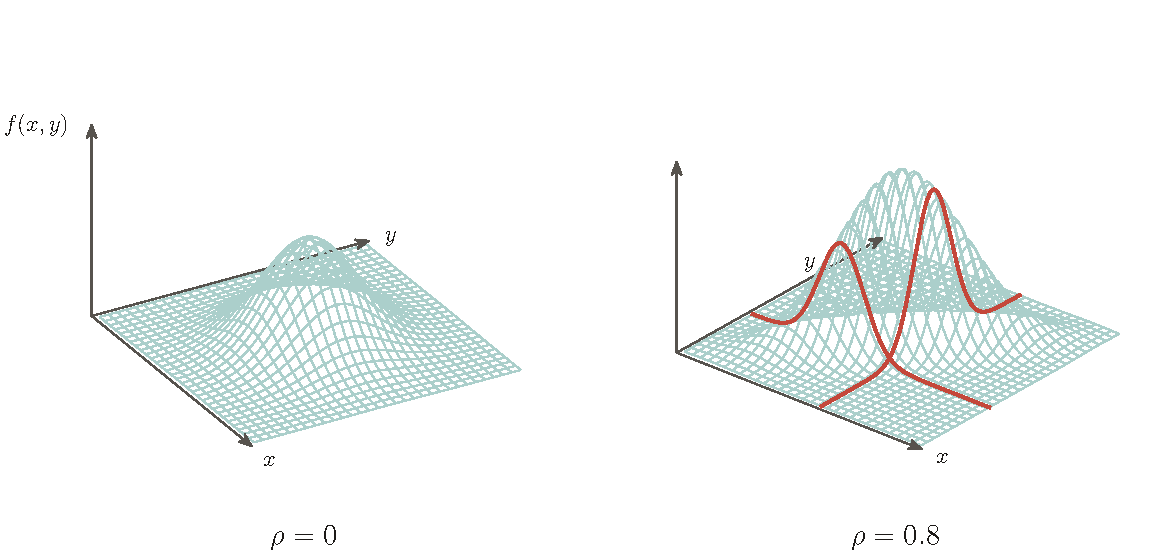
\includegraphics[width=0.92\textwidth]{normal-bivariada-rho.pdf}
\caption{Densidades normais bivariadas padrão para $\rho=0$ (à esquerda) e
$\rho=0{,}8$ (à direita), na mesma escala vertical. Para $\rho=0$, a superfície é radialmente
simétrica; para $\rho=0{,}8$, a malha se alonga na direção $y=x$.
As curvas vermelhas destacam as seções $x=1/2$ e $y=-1$ da densidade conjunta;
para obter as densidades condicionais, dividimos cada seção pela marginal correspondente.}
\label{fig:normal-bivariada-rho}
\end{figure}
Essa função é não negativa. Que sua integral sobre $\mathbb{R}^2$ vale $1$ é verificado no
\Cref{exercise:normalizacao-bivariada}, ao final da subseção, como consequência dos cálculos
a seguir. Dizemos que $(X,Y)$ tem \emph{distribuição normal bivariada padrão} com parâmetro
$\rho$ quando sua densidade conjunta é \eqref{eq:normal-bivariada-padrao}. Para obter a
densidade condicional, precisamos da marginal de $X$. Para isso, completamos o quadrado no
expoente, uma técnica que reaparece em todos os cálculos com a normal bivariada.

\begin{proposition}[Densidade condicional da normal bivariada padrão]
\label{prop:normal-bivariada}
Suponha que $(X,Y)$ tenha densidade conjunta dada por
\eqref{eq:normal-bivariada-padrao}. Então a densidade marginal de $X$ é a densidade normal
padrão
\begin{equation}
  f_X(x) = \frac{1}{\sqrt{2\pi}} e^{-x^2/2}, \qquad x \in \mathbb{R},
  \label{eq:marginal-normal-padrao}
\end{equation}
e, para cada $x \in \mathbb{R}$, a densidade condicional de $Y$ dado $X = x$ é
\begin{equation}
  f_{Y\mid X}(y \mid x)
  = \frac{1}{\sqrt{2\pi(1-\rho^2)}}
  \exp\!\left(-\frac{(y-\rho x)^2}{2(1-\rho^2)}\right),
  \qquad y \in \mathbb{R}.
  \label{eq:condicional-normal-padrao}
\end{equation}
Em outras palavras, a distribuição condicional de $Y$ dado $X = x$ é $N(\rho x,\, 1-\rho^2)$,
isto é, normal de média $\rho x$ e variância $1-\rho^2$.
\end{proposition}

\begin{proof}
Por definição, $f_X(x) = \int_{-\infty}^{\infty} f(x,y)\,dy$. Completando o quadrado em $y$,
obtemos
\[
  x^2 - 2\rho xy + y^2 = (y - \rho x)^2 + x^2(1-\rho^2).
\]
Ao dividir pelo fator $2(1-\rho^2)$ do denominador do expoente, a parcela $x^2(1-\rho^2)$
se reduz a $x^2/2$, que não depende de $y$. Usando $e^{a+b} = e^a e^b$, a dependência em $x$
se separa no produto $\exp(-x^2/2)\exp\!\left(-\frac{(y-\rho x)^2}{2(1-\rho^2)}\right)$. A
exponencial que depende de $x$ sai da integral em $y$ e, multiplicando e dividindo por
$\sqrt{2\pi(1-\rho^2)}$, reconhecemos a densidade de $N(\rho x, 1-\rho^2)$:
\begin{align*}
  f_X(x)
  &= \frac{1}{2\pi\sqrt{1-\rho^2}}
     \exp\!\left(-\frac{x^2}{2}\right)
     \int_{-\infty}^{\infty}
     \exp\!\left(-\frac{(y-\rho x)^2}{2(1-\rho^2)}\right)\,dy \\[0.3cm]
  &= \frac{1}{\sqrt{2\pi}}\exp\!\left(-\frac{x^2}{2}\right)
     \underbrace{\int_{-\infty}^{\infty}\frac{1}{\sqrt{2\pi(1-\rho^2)}}
     \exp\!\left(-\frac{(y-\rho x)^2}{2(1-\rho^2)}\right)\,dy}_{=\,1}.
\end{align*}
O integrando destacado é a densidade de $N(\rho x, 1-\rho^2)$ na variável $y$, logo sua
integral vale $1$, e segue \eqref{eq:marginal-normal-padrao}. Como $f_X(x) > 0$ para todo
$x \in \mathbb{R}$, podemos dividir a densidade conjunta por $f_X(x)$ em todos os pontos.
Dividindo por \eqref{eq:marginal-normal-padrao}, os fatores $\exp(-x^2/2)$ se cancelam e
resta
\[
  f_{Y\mid X}(y \mid x)
  = \frac{f_{X,Y}(x,y)}{f_X(x)}
  = \frac{1}{\sqrt{2\pi(1-\rho^2)}}
    \exp\!\left(-\frac{(y-\rho x)^2}{2(1-\rho^2)}\right),
\]
que é \eqref{eq:condicional-normal-padrao}.
\end{proof}

\begin{remark}[Caso geral e independência]\label{rem:normal-independencia}
Sejam $\mu_1,\mu_2 \in \mathbb{R}$, $\sigma_1,\sigma_2 > 0$ e $\rho \in (-1,1)$. Dizemos que
$(X,Y)$ tem \emph{distribuição normal bivariada} com esses parâmetros quando sua densidade
conjunta é
\begin{equation}
  g(x,y) = \frac{1}{2\pi\sigma_1\sigma_2\sqrt{1-\rho^2}}
  \exp\!\left(-\frac{Q(x,y)}{2}\right),
  \qquad (x,y) \in \mathbb{R}^2,
  \label{eq:normal-bivariada-geral}
\end{equation}
onde $Q$ é a expressão quadrática
\begin{equation}
  Q(x,y) = \frac{1}{1-\rho^2}\left[
    \left(\frac{x-\mu_1}{\sigma_1}\right)^2
    - 2\rho\left(\frac{x-\mu_1}{\sigma_1}\right)
         \left(\frac{y-\mu_2}{\sigma_2}\right)
    + \left(\frac{y-\mu_2}{\sigma_2}\right)^2
  \right].
  \label{eq:forma-quadratica-normal}
\end{equation}
O caso padrão corresponde a $\mu_1 = \mu_2 = 0$ e $\sigma_1 = \sigma_2 = 1$, pois então
$Q(x,y) = (x^2 - 2\rho xy + y^2)/(1-\rho^2)$, e $-Q(x,y)/2$ é o expoente de
\eqref{eq:normal-bivariada-padrao}.

Para reduzir o caso geral ao padrão, definimos
\[
  U = \frac{X-\mu_1}{\sigma_1}, \qquad V = \frac{Y-\mu_2}{\sigma_2}.
\]
A transformação inversa é $x = \mu_1 + \sigma_1 u$ e $y = \mu_2 + \sigma_2 v$. Sua matriz
jacobiana é diagonal, com entradas $\sigma_1$ e $\sigma_2$, de modo que o jacobiano vale
$\sigma_1\sigma_2$. Pela fórmula da densidade de uma transformação afim de um par de
variáveis com densidade, vista nas notas sobre somas de variáveis aleatórias contínuas e
mudança de variáveis, a densidade de $(U,V)$ é
\[
  g(\mu_1 + \sigma_1 u,\, \mu_2 + \sigma_2 v)\,\sigma_1\sigma_2
  = \frac{1}{2\pi\sqrt{1-\rho^2}}
    \exp\!\left(-\frac{u^2 - 2\rho uv + v^2}{2(1-\rho^2)}\right),
\]
que é exatamente \eqref{eq:normal-bivariada-padrao}. Logo, $(U,V)$ tem distribuição normal
bivariada padrão e, pela \Cref{prop:normal-bivariada}, a distribuição condicional de $V$ dado
$U = u$ é $N(\rho u, 1-\rho^2)$.

Como $Y = \mu_2 + \sigma_2 V$, a densidade condicional de $Y$ dado $X = x$ é obtida da de
$V$ dado $U = u$, com $u = (x-\mu_1)/\sigma_1$, pela mesma transformação afim unidimensional:
ela divide a densidade por $\sigma_2$ e troca $v$ por $(y-\mu_2)/\sigma_2$. Obtemos
\begin{equation}
  f_{Y\mid X}(y \mid x)
  = \frac{1}{\sqrt{2\pi\sigma_2^2(1-\rho^2)}}
    \exp\!\left(
      -\frac{\left(y - \mu_2 - \rho\sigma_2(x-\mu_1)/\sigma_1\right)^2}
            {2\sigma_2^2(1-\rho^2)}
    \right).
  \label{eq:condicional-normal-geral}
\end{equation}
A distribuição condicional de $Y$ dado $X = x$ é, portanto, normal, com média
$\mu_2 + \rho\sigma_2(x-\mu_1)/\sigma_1$ e variância $\sigma_2^2(1-\rho^2)$. A média
condicional é afim em $x$, e a variância não depende de $x$.

Quanto à independência, se $\rho = 0$, então \eqref{eq:normal-bivariada-geral} se fatoriza
como o produto das densidades de $N(\mu_1,\sigma_1^2)$ e $N(\mu_2,\sigma_2^2)$;
logo, $X$ e $Y$ são independentes. Reciprocamente, se $X$ e $Y$ são independentes,
a distribuição condicional de $Y$ dado $X=x$ coincide com a marginal de $Y$
para quase todo $x$. Sua média deve, portanto, ser constante em $x$.
Como a média condicional é $\mu_2+\rho\sigma_2(x-\mu_1)/\sigma_1$,
com $\sigma_1,\sigma_2>0$, isso força $\rho=0$. Assim, no caso
normal, $X$ e $Y$ são independentes se, e somente se, $\rho = 0$. Fora do caso normal, essa
equivalência pode falhar: há variáveis com covariância nula que não são independentes, o que
será discutido no estudo da covariância e da correlação.
\end{remark}

\begin{exercise}[Normalização da densidade normal bivariada]
\label{exercise:normalizacao-bivariada}
Mostre que a função $f$ definida em \eqref{eq:normal-bivariada-padrao} integra $1$ sobre
$\mathbb{R}^2$. Sugestão: integre primeiro na variável $y$, use
o cálculo da integral em $y$ na prova da \Cref{prop:normal-bivariada}
para identificar a integral interna e lembre que a normal
padrão tem integral $1$. Não é preciso refazer a integral gaussiana.
\end{exercise}

\subsection{Uma Densidade Uniforme em um Triângulo}\label{subsec:uniforme-triangulo}

No primeiro exemplo desta seção, o suporte era ilimitado e a densidade conjunta decaía
exponencialmente. Vamos agora considerar uma região limitada e uma densidade conjunta
constante, para ver como o formato do suporte se reflete na densidade condicional. Seja
\[
  D = \bigl\{(x,y) \in \mathbb{R}^2 : x \geqslant 0,\ y \geqslant 0,\ x+y \leqslant 1\bigr\}
\]
o triângulo de vértices $(0,0)$, $(1,0)$ e $(0,1)$, cuja área é $1/2$.

\begin{example}[Uniforme em um triângulo]\label{ex:uniforme-triangulo}
Suponha que $(X,Y)$ tenha distribuição uniforme sobre $D$, isto é, que sua densidade
conjunta seja
\begin{equation}\label{eq:uniforme-triangulo-conjunta}
  f_{X,Y}(x,y) =
  \begin{cases}
    2, & \text{se } x>0,\ y>0,\ x+y<1, \\
    0, & \text{caso contrário}.
  \end{cases}
\end{equation}
O valor constante $2$ não é arbitrário: a densidade de uma distribuição uniforme sobre uma
região plana é o inverso da área dessa região, e aqui $1/(1/2) = 2$.
Como a fronteira de $D$ tem área zero, atribuir o valor $0$ à densidade
nessa fronteira não altera as probabilidades. Determine a densidade
marginal de $X$ e a densidade condicional de $Y$ dado $X = x$; em seguida, calcule
$\mathbb{P}(Y \leqslant 1/4 \mid X = 1/2)$.
\end{example}

\begin{solution}
Fixado $x$ com $0 < x < 1$, a seção vertical do triângulo na abscissa $x$ é o intervalo
$[0,1-x]$, de comprimento $1-x$. A densidade é positiva no interior desse intervalo
e se anula nas extremidades. Integrando a densidade conjunta nessa seção,
obtemos
\begin{equation}\label{eq:marginal-x-uniforme-triangulo}
  f_X(x) = \int_0^{1-x} 2\,dy = 2(1-x),
\end{equation}
e $f_X(x) = 0$ fora do intervalo $(0,1)$. Conferimos a normalização:
\[
  \int_0^1 2(1-x)\,dx = 2\Bigl[x - \frac{x^2}{2}\Bigr]_0^1 = 1.
\]
Note que $f_X$ decresce linearmente em $x$: as seções verticais do triângulo encurtam quando
$x$ se aproxima de $1$, e a marginal herda esse comportamento.

Com a marginal em mãos, a densidade condicional é o quociente $f_{X,Y}(x,y)/f_X(x)$,
definido para os $x$ com $f_X(x) > 0$, isto é, para $0 < x < 1$. Para $0 < y < 1-x$, o ponto
$(x,y)$ está em $D$, de modo que $f_{X,Y}(x,y) = 2$, e portanto
\begin{equation}\label{eq:condicional-uniforme-triangulo}
  f_{Y\mid X}(y \mid x) = \frac{2}{2(1-x)} = \frac{1}{1-x},
\end{equation}
enquanto $f_{Y\mid X}(y \mid x) = 0$ fora do intervalo $(0,1-x)$. A normalização é imediata:
\[
  \int_0^{1-x} \frac{1}{1-x}\,dy = \frac{1}{1-x}\int_0^{1-x} dy = 1.
\]
Logo, dado $X = x$, a distribuição condicional de $Y$ é uniforme no intervalo $(0,1-x)$. A
leitura geométrica é direta: condicionar em $X = x$ equivale a cortar o triângulo pela reta
vertical de abscissa $x$ e olhar a distribuição sobre o segmento restante, de comprimento
$1-x$. Como a densidade conjunta é constante sobre $D$, a distribuição ao longo desse
segmento é uniforme.

Por simetria, trocando os papéis de $x$ e $y$, obtemos, para $0 < y < 1$ e $0 < x < 1-y$, a
densidade $f_{X\mid Y}(x \mid y) = 1/(1-y)$. Ou seja, dado $Y = y$, a distribuição
condicional de $X$ é uniforme em $(0,1-y)$.

Para calcular a probabilidade pedida, fixamos $x = 1/2$. Então $1-x = 1/2$ e a densidade
condicional vale $2$ no intervalo $(0,1/2)$. Pela definição de
$\mathbb{P}(Y \leqslant y \mid X = x)$, essa probabilidade é a integral da densidade
condicional sobre $(-\infty, 1/4]$:
\[
  \mathbb{P}\Bigl(Y \leqslant \frac{1}{4} \,\Bigm|\, X = \frac{1}{2}\Bigr)
  = \int_0^{1/4} \frac{1}{1/2}\,dy = 2 \cdot \frac{1}{4} = \frac{1}{2}.
\]
O resultado é coerente: dado $X = 1/2$, o segmento disponível para $Y$ tem comprimento
$1/2$, e até $y = 1/4$ percorremos a metade dele.
\end{solution}

O exemplo ilustra um mecanismo geral. Ao integrar a densidade conjunta, que é constante,
sobre a seção vertical, o resultado é essa constante vezes o comprimento da seção. Assim, o
fator $2$ é a densidade uniforme sobre $D$ e o fator $(1-x)$ é o comprimento da seção, o que
deu $f_X(x) = 2(1-x)$. Quando a densidade conjunta é constante, a marginal de $X$ é
proporcional ao comprimento das seções verticais. Ao formar a razão que define a densidade
condicional, a constante da densidade conjunta se cancela, restando o inverso
do comprimento da seção, que é uma densidade constante sobre a
seção. Esse mesmo mecanismo aparece nas notas sobre vetores contínuos, no cálculo das
marginais de uniformes sobre retângulos.

\section{Exercícios}\label{sec:exercicios-condicionais}

Reunimos aqui dois exercícios resolvidos, que retomam o cálculo da densidade condicional em
outros domínios triangulares. A receita é, em geral, a mesma: determinar as marginais,
dividir a densidade conjunta pela marginal apropriada e, por fim, conferir a normalização
do resultado. Os dois exercícios complementares, na seção seguinte, tratam da uniforme no
disco e de um modelo em que a densidade condicional de $Y$ dado $X = x$ é especificada
diretamente.

\begin{exercise}[Condicionais em outro domínio triangular]\label{exercise:condicional-exponencial}
Suponha que $X$ e $Y$ tenham densidade conjunta
\begin{equation}
  f_{X,Y}(x,y) =
  \begin{cases}
    e^{-y}, & \text{se } 0 < x < y < \infty, \\[0.2cm]
    0, & \text{caso contrário}.
  \end{cases}
  \label{eq:densidade-exercicio-660}
\end{equation}
Determine as densidades condicionais de $Y$ dado $X = x$ e de $X$ dado $Y = y$.
\end{exercise}

\begin{solution}
Antes de começar, observe que o suporte da densidade conjunta é o triângulo
$\{(x,y) : 0 < x < y < \infty\}$. Sobre esse conjunto, $f_{X,Y}$ é positiva, e fora dele
vale $0$. Como as duas densidades condicionais se obtêm dividindo a conjunta pela marginal
correspondente, começamos determinando as duas marginais.

\noindent\textbf{Densidade marginal de $X$.}
Fixado $x > 0$, a variável $y$ percorre o intervalo $(x,\infty)$. Assim, integrando a
conjunta em $y$, obtemos
\begin{equation}
  f_X(x) = \int_{-\infty}^{\infty} f_{X,Y}(x,y)\,dy
  = \int_x^{\infty} e^{-y}\,dy
  = \bigl[-e^{-y}\bigr]_{y=x}^{\infty}
  = e^{-x},
  \label{eq:marginal-x-660}
\end{equation}
para $x > 0$, e $f_X(x) = 0$ se $x \leqslant 0$. Essa é a densidade de uma variável
exponencial de parâmetro $1$.

\noindent\textbf{Densidade marginal de $Y$.}
Fixado $y > 0$, a variável $x$ percorre o intervalo $(0,y)$. Como o integrando $e^{-y}$ não
depende de $x$, a integral é imediata:
\begin{equation}
  f_Y(y) = \int_{-\infty}^{\infty} f_{X,Y}(x,y)\,dx
  = \int_0^{y} e^{-y}\,dx
  = y\,e^{-y},
  \label{eq:marginal-y-660}
\end{equation}
para $y > 0$, e $f_Y(y) = 0$ se $y \leqslant 0$. Reconhecemos em $f_Y$ a densidade
$\mathrm{Gama}(2,1)$, que também é a densidade da soma de duas variáveis exponenciais
independentes de parâmetro $1$, como estudado nas notas sobre somas de variáveis aleatórias
contínuas. Isso não é coincidência. No suporte, $f_{X,Y}(x,y) = e^{-x}\,e^{-(y-x)}$, o que
mostra, pela mudança de variáveis $(x,y) \mapsto (x,\, y-x)$ (de jacobiano $1$), que $X$ e
$Y-X$ são independentes e exponenciais de parâmetro $1$. Logo, $Y = X + (Y-X)$ é uma soma
desse tipo. A presença do fator $y$ é o que distingue $f_Y$ de $f_X$, cuja forma é apenas
$e^{-x}$.

\noindent\textbf{Condicional de $Y$ dado $X = x$.}
Fixe $x > 0$, de modo que $f_X(x) = e^{-x} > 0$. Dividindo a conjunta pela marginal em $x$,
obtemos
\begin{equation}
  f_{Y\mid X}(y \mid x)
  = \frac{f_{X,Y}(x,y)}{f_X(x)}
  = \frac{e^{-y}}{e^{-x}}
  = e^{-(y-x)},
  \label{eq:condicional-y-x-660}
\end{equation}
para $y > x$, e $f_{Y\mid X}(y \mid x) = 0$ caso contrário. Vamos conferir a normalização.
Substituindo $u = y - x$, de modo que $dy = du$ e os limites $y > x$ se tornam $u > 0$,
\[
  \int_x^{\infty} e^{-(y-x)}\,dy
  = \int_0^{\infty} e^{-u}\,du
  = 1.
\]
Portanto, $f_{Y\mid X}(\cdot \mid x)$ é de fato uma densidade de probabilidade sobre
$(x,\infty)$. Reconhecemos nela uma exponencial de parâmetro $1$ deslocada em $x$.

\noindent\textbf{Condicional de $X$ dado $Y = y$.}
Fixe $y > 0$, de modo que $f_Y(y) = y\,e^{-y} > 0$. Dividindo a conjunta pela marginal em
$y$, encontramos
\begin{equation}
  f_{X\mid Y}(x \mid y)
  = \frac{f_{X,Y}(x,y)}{f_Y(y)}
  = \frac{e^{-y}}{y\,e^{-y}}
  = \frac{1}{y},
  \label{eq:condicional-x-y-660}
\end{equation}
para $0 < x < y$, e $f_{X\mid Y}(x \mid y) = 0$ caso contrário. A normalização também é
imediata, pois o integrando é constante no intervalo de integração:
\[
  \int_0^{y} \frac{1}{y}\,dx
  = \frac{1}{y}\cdot y
  = 1.
\]
Logo, $f_{X\mid Y}(\cdot \mid y)$ é a densidade da distribuição uniforme no intervalo $(0,y)$.

Por fim, interpretemos o resultado. A igualdade em \eqref{eq:condicional-x-y-660} diz que,
uma vez dado $Y = y$, a variável $X$ não tem preferência por nenhum ponto de $(0,y)$: ela é
uniforme ali. Vale comparar com o \Cref{ex:dominio-triangular}, no qual
a conjunta era $2e^{-x-y}$ e a condicional de $X$ dado $Y = y$ resultava ser a exponencial
truncada $e^{-x}/(1-e^{-y})$, concentrada perto de $x = 0$. A diferença está na conjunta.
Lá, $f_{X,Y}(x,y) = 2e^{-x-y}$ depende de $x$, e essa dependência sobrevive na condicional.
Aqui, $f_{X,Y}(x,y) = e^{-y}$ não depende de $x$ sobre o suporte. Como $f_Y(y)$ também não
depende de $x$, a condicional de $X$ dado $Y = y$ é constante em $x$, isto é, uniforme.
\end{solution}

\begin{exercise}[Posição de $X$ dado o valor da soma]\label{exercise:uniforme-dado-soma}
Sejam $X$ e $Y$ variáveis aleatórias independentes, cada uma com distribuição exponencial de
parâmetro $\lambda > 0$. Determine a densidade conjunta de $X$ e de $X+Y$ e deduza que a
densidade condicional de $X$ dado que $X+Y = a$ é uniforme no intervalo $(0,a)$, para cada
$a > 0$. Interprete o resultado: saber que $X+Y = a$ restringe $X$ ao intervalo $(0,a)$, mas
não favorece nenhum ponto desse intervalo.
\end{exercise}

\begin{solution}
Como $X$ e $Y$ são independentes e ambas têm distribuição $\mathrm{Exp}(\lambda)$, a densidade
conjunta de partida é
\begin{equation}\label{eq:densidade-exercicio-661}
  f_{X,Y}(x,y) = \lambda e^{-\lambda x}\,\lambda e^{-\lambda y}
  = \lambda^2 e^{-\lambda x}e^{-\lambda y},
\end{equation}
para $x > 0$ e $y > 0$, e $f_{X,Y}(x,y) = 0$ caso contrário.

Passamos da descrição pelas coordenadas $(X,Y)$ para a descrição pelas coordenadas $(U,V)$,
com
\[
  U = X, \qquad V = X + Y.
\]
A segunda coordenada é justamente a soma que queremos estudar. Invertendo o sistema,
obtemos $x = u$ e $y = v - u$. Assim, as condições $x > 0$ e $y > 0$ se traduzem em
$0 < u < v$, que é a imagem do suporte pela transformação. Para aplicar a fórmula de mudança
de variáveis, calculamos o determinante jacobiano da aplicação inversa $(u,v) \mapsto (x,y)$.
As derivadas parciais são
\[
  \frac{\partial x}{\partial u} = 1, \quad
  \frac{\partial x}{\partial v} = 0, \quad
  \frac{\partial y}{\partial u} = -1, \quad
  \frac{\partial y}{\partial v} = 1,
\]
e portanto
\[
  J = \det
  \begin{pmatrix}
    \dfrac{\partial x}{\partial u} \ & \dfrac{\partial x}{\partial v} \\[0.5cm]
    \dfrac{\partial y}{\partial u} \ & \dfrac{\partial y}{\partial v}
  \end{pmatrix}
  = \det \begin{pmatrix} 1 & 0 \\ -1 & 1 \end{pmatrix}
  = 1 \cdot 1 - 0 \cdot (-1) = 1.
\]
Como $|J| = 1$, a mudança de variáveis preserva áreas infinitesimais. Substituindo $x = u$ e
$y = v-u$ em \eqref{eq:densidade-exercicio-661} e multiplicando por $|J| = 1$, obtemos, para
$0 < u < v$,
\[
  f_{U,V}(u,v) = f_{X,Y}(u, v-u) = \lambda^2 e^{-\lambda u}e^{-\lambda (v-u)}.
\]
O ponto-chave está na simplificação dos expoentes:
\[
  e^{-\lambda u}\,e^{-\lambda (v-u)} = e^{-\lambda u - \lambda v + \lambda u}
  = e^{-\lambda v},
\]
isto é, os termos que dependem de $u$ se cancelam. Assim, no suporte $0<u<v$,
o valor da densidade conjunta de $(U,V)$ depende apenas de $v$:
\begin{equation}\label{eq:conjunta-x-soma}
  f_{U,V}(u,v) =
  \begin{cases}
    \lambda^2 e^{-\lambda v}, & \text{se } 0 < u < v, \\[0.2cm]
    0, & \text{caso contrário}.
  \end{cases}
\end{equation}

\begin{figure}[H]
\centering
\begin{tikzpicture}[scale=0.9, >=Stealth]
  % O suporte é ilimitado; a janela apenas limita o trecho desenhado.
  \path[use as bounding box] (-0.6,-0.5) rectangle (5.3,5.3);
  \begin{scope}
    \clip (-0.6,-0.5) rectangle (5.3,5.3);
    \fill[teal!15] (0,0) -- (0,6) -- (6,6) -- cycle;
  \end{scope}

  % Eixos e fronteira aberta do suporte.
  \draw[->, thick] (-0.5,0) -- (5.1,0) node[below] {$u$};
  \draw[->, thick] (0,-0.4) -- (0,5.1) node[left] {$v$};
  \draw[thick, muted, dashed] (0,0) -- (5.2,5.2);
  \node[below left=2pt] at (0,0) {$0$};

  % Seção vertical para u=u_0: v>u_0, sem limite superior na janela.
  \draw[red!75, dashed] (1.15,0) -- (1.15,1.15);
  \draw[red!75, thick] (1.15,1.15) -- (1.15,5.3);
  \draw[red!75, thick, fill=white] (1.15,1.15) circle (2pt);
  \draw[muted] (1.15,0) -- (1.15,-0.12);
  \node[below=3pt] at (1.15,0) {$u_0$};

  % Seção horizontal para v=v_0: 0<u<v_0.
  \draw[red!75, dashed] (3.1,0) -- (3.1,3.1);
  \draw[red!75, thick] (0,3.1) -- (3.1,3.1);
  \draw[red!75, thick, fill=white] (0,3.1) circle (2pt);
  \draw[red!75, thick, fill=white] (3.1,3.1) circle (2pt);
  \draw[muted] (0,3.1) -- (-0.12,3.1);
  \node[left=3pt] at (0,3.1) {$v_0$};
  \draw[muted] (3.1,0) -- (3.1,-0.12);
  \node[below=3pt] at (3.1,0) {$v_0$};
\end{tikzpicture}
\caption{O suporte $S=\{(u,v):0<u<v\}$, sombreado, é verticalmente simples e
horizontalmente simples. As seções destacadas em vermelho correspondem, respectivamente,
a $u=u_0$, com $u_0<v<\infty$, e a $v=v_0$, com $0<u<v_0$; a seção vertical continua
além da janela desenhada.}
\label{fig:suporte-transformado}
\end{figure}

Para cada $v$ fixo, a expressão $\lambda^2 e^{-\lambda v}$ não depende de $u$: sobre o
triângulo $0 < u < v$, a densidade conjunta tem sempre a mesma altura, e toda a variação
fica por conta de $v$.

Passamos à marginal de $V = X+Y$, integrando \eqref{eq:conjunta-x-soma} em $u$ sobre o
suporte compatível. Fixado $v > 0$, a variável $u$ percorre $(0,v)$ e o integrando não
depende de $u$, de modo que
\begin{equation}\label{eq:marginal-soma-661}
  f_V(v) = \int_{0}^{v} \lambda^2 e^{-\lambda v}\,du
  = \lambda^2 e^{-\lambda v} \int_{0}^{v} du
  = \lambda^2 v e^{-\lambda v},
\end{equation}
para $v > 0$, e $f_V(v) = 0$ caso contrário. Reconhecemos em \eqref{eq:marginal-soma-661} a
densidade de uma $\mathrm{Gama}(2,\lambda)$, pois a forma geral é
$\lambda^{\alpha} v^{\alpha-1} e^{-\lambda v}/\Gamma(\alpha)$, com $\alpha = 2$ e
$\Gamma(2) = 1$. Esse é o mesmo resultado que obteríamos pela fórmula da convolução para a
soma de duas exponenciais independentes, vista nas notas sobre somas de variáveis aleatórias
contínuas.

Finalmente, calculamos a densidade condicional. Para $0 < u < v$ temos $f_V(v) > 0$, de modo
que a definição se aplica e
\begin{equation}\label{eq:condicional-uniforme-661}
  f_{U\mid V}(u \mid v)
  = \frac{f_{U,V}(u,v)}{f_V(v)}
  = \frac{\lambda^2 e^{-\lambda v}}{\lambda^2 v e^{-\lambda v}}
  = \frac{1}{v},
\end{equation}
enquanto $f_{U\mid V}(u \mid v) = 0$ fora do intervalo $(0,v)$. O cancelamento de
$\lambda^2 e^{-\lambda v}$ mostra que a densidade condicional é uniforme em $(0,v)$, qualquer
que seja $v>0$. Sua normalização é $\int_0^v (1/v)\,du=1$.
Traduzindo para as variáveis originais, dado que $X+Y = a$ com $a > 0$,
\[
  f_{U\mid V}(u \mid a) = \frac{1}{a} \quad \text{para } 0 < u < a,
\]
isto é, a distribuição condicional de $X = U$ dado $X+Y = a$ é uniforme no intervalo $(0,a)$.

A interpretação é a esperada. Saber que a soma vale $a$ informa que $X$ está em $(0,a)$, mas
não privilegia nenhum ponto desse intervalo: a densidade condicional é constante e igual a
$1/a$, a altura necessária para que a área total seja $1$. O resultado também tem
uma interpretação em termos de chegadas: se o instante da primeira chegada
e o intervalo entre as duas chegadas são independentes e exponenciais, então, sabendo apenas
o instante da segunda chegada, o instante da primeira é uniforme no intervalo $(0,a)$.
\end{solution}

\section{Exercícios Complementares}\label{sec:exercicios-complementares}

Os exercícios a seguir aplicam a fórmula da densidade condicional a dois modelos concretos.
No primeiro, a densidade conjunta é dada, e basta obter a marginal e a condicional. No
segundo, a densidade condicional é dada, e é preciso primeiro obter a conjunta. Em ambos,
justifique cada passo.

\begin{exercise}[Uniforme no disco]\label{exercise:disco-uniforme}
Seja $(X,Y)$ um vetor aleatório uniformemente distribuído sobre o disco unitário
$D = \{(x,y) : x^2 + y^2 \leqslant 1\}$, de área $\pi$, isto é,
\begin{equation}\label{eq:uniforme-disco}
  f_{X,Y}(x,y) =
  \begin{cases}
    \dfrac{1}{\pi}, & \text{se } x^2+y^2<1, \\[0.3cm]
    0, & \text{caso contrário}.
  \end{cases}
\end{equation}
Escolhemos o valor $0$ na circunferência que delimita $D$, pois ela tem área zero.
Faça o que se pede.

\begin{enumerate}
  \item[(a)] Mostre que
  \begin{equation}\label{eq:marginal-x-disco}
    f_X(x) = \frac{2}{\pi}\sqrt{1-x^2}, \qquad x \in (-1,1),
  \end{equation}
  e que $f_X(x) = 0$ fora desse intervalo.

  \item[(b)] Mostre que, para $x \in (-1,1)$,
  \begin{equation}\label{eq:condicional-disco}
    f_{Y\mid X}(y \mid x)
    = \frac{1}{2\sqrt{1-x^2}}, \qquad
    y \in \bigl(-\sqrt{1-x^2}, \sqrt{1-x^2}\bigr),
  \end{equation}
  e que $f_{Y\mid X}(y \mid x) = 0$ fora desse intervalo.

  \item[(c)] Conclua e comente: dado $X = x$, a variável $Y$ é uniforme no segmento vertical
  de comprimento $2\sqrt{1-x^2}$ que constitui a seção do disco pela reta vertical de
  abscissa $x$.
\end{enumerate}

\emph{Sugestão.} Para obter a marginal de $X$, integre $1/\pi$ na vertical: a seção do disco
pela reta de abscissa $x$ tem comprimento $2\sqrt{1-x^2}$. A condicional é o quociente entre
a densidade conjunta e a marginal, definida apenas para $x$ com $f_X(x) > 0$.
\end{exercise}

\begin{exercise}[Um modelo em duas etapas]\label{exercise:modelo-duas-etapas}
Seja $X$ uniforme no intervalo $(0,1)$. Suponha que, dado $X = x$, a variável $Y$ seja
uniforme no intervalo $(0,x)$, de modo que a densidade condicional de $Y$ dado $X = x$ é
\[
  f_{Y\mid X}(y \mid x) = \frac{1}{x}, \qquad 0 < y < x < 1.
\]
Faça o que se pede.

\begin{enumerate}
  \item[(a)] Mostre que a densidade conjunta de $(X,Y)$ é
  \begin{equation}\label{eq:conjunta-hierarquico}
    f_{X,Y}(x,y) =
    \begin{cases}
      \dfrac{1}{x}, & \text{se } 0 < y < x < 1, \\[0.5cm]
      0, & \text{caso contrário}.
    \end{cases}
  \end{equation}

  \item[(b)] Integre em $x$ para mostrar que a densidade marginal de $Y$ é
  \begin{equation}\label{eq:marginal-y-hierarquico}
    f_Y(y) = -\ln y, \qquad y \in (0,1),
  \end{equation}
  e que $f_Y(y) = 0$ fora desse intervalo.

  \item[(c)] Mostre que, para $y \in (0,1)$,
  \begin{equation}\label{eq:condicional-hierarquico}
    f_{X\mid Y}(x \mid y) = \frac{1}{x\,(-\ln y)}, \qquad x \in (y,1),
  \end{equation}
  e que $f_{X\mid Y}(x \mid y) = 0$ fora desse intervalo.
\end{enumerate}

\noindent\emph{Sugestão.} Use a definição de densidade condicional na forma
\[
  f_{X,Y}(x,y) = f_{Y\mid X}(y \mid x)\, f_X(x),
\]
isto é, multiplique a densidade condicional
de $Y$ dado $X = x$ pela densidade marginal de $X$ para obter a conjunta. Depois, integre em
$x$ para obter a marginal de $Y$ e, por fim, aplique novamente a definição de densidade
condicional.
\end{exercise}


\bibliographystyle{plain}
\bibliography{../arquivos-aux/referencias}
\end{document}
